\subsection{VGG ESDs and the Trace Log Condition}
\begin{figure}[t]
    \centering
    \subfigure[VGG19 layer FC1 ESD]{
      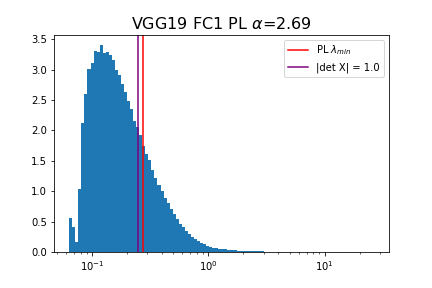
\includegraphics[width=6cm]{./img/VGG19_FC1.png}
    }
    \subfigure[VGG19 layer FC3 ESD]{
      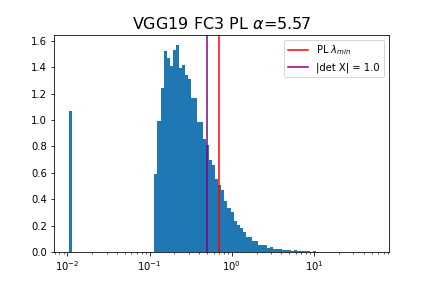
\includegraphics[width=6cm]{./img/VGG19_FC3.png}
    }
    \caption{Comparison of \WW~PL fit $\LAMBDAPL$ (in red) with the $\LAMBDADETX$ that best fits the Trace Log 
        Condition $\left(\vert \det \mathbf{X}^{eff}\vert = 1\right)$, (purple), for the FC1 and FC3 layers in VGG11. In 
        both cases, $\LAMBDAPL - \LAMBDADETX$ is small, and positive, i.e. the red line is slightly to the right of the 
        purple line.
    }
  \label{fig:VGG11_esds}
\end{figure}

Figure~\ref{fig:VGG11_esds} displays the layer ESD from the FC1 and FC3 layers from
the widely available, pre-trained VGG19 model
\footnote{We used the VGG19 model as distributed in torchvision python package version (with the ImageNetV1 dataset).}.
The \WW~PL fit gives $\alpha=2.40$, for FC1, and $\alpha=2.98$, for FC3. (See also \cite{MM18_TR_JMLRversion}.)
As above, the red and purple lines nearly overlap when $\alpha\simeq 2.0$,
and pull farther apart as $\alpha$ increases.
However, the lines are closer together for VGG16 than for the MLP3 FC1 layer, (except for when $lr=16\times$ normal and 
$\LAMBDAPL < \LAMBDADETX$,) even for much larger values of $\alpha_{VGG}$.
This suggests that for SOTA models, at least in some cases, the Trace Log of
the weight matrices may be near zero in very many cases.
